\documentclass[11pt]{article}

\usepackage[english]{babel}
\usepackage[utf8]{inputenc}
\usepackage[T1]{fontenc}
\usepackage{lmodern}
\usepackage{microtype}
\usepackage{amsmath,amssymb,amsthm,mathtools,amscd}
\usepackage[a4paper,margin=1in]{geometry}
\usepackage{parskip}
\usepackage{enumitem}
\usepackage{xcolor}
\usepackage{hyperref}
\usepackage{tikz}
\usetikzlibrary{arrows.meta,positioning,fit,calc,backgrounds}

\hypersetup{colorlinks=true,linkcolor=blue,citecolor=blue,urlcolor=blue}

\newcommand{\R}{\mathbb{R}}
\newcommand{\Z}{\mathbb{Z}}
\newcommand{\Q}{\mathbb{Q}}
\newcommand{\kk}{\Bbbk}
\newcommand{\TAMER}{\textsc{TAMER-OP}}
\newcommand{\multipers}{\textsc{multipers}}
\newcommand{\bbb}[1]{\mathbb{#1}}

\newtheorem{theorem}{Theorem}
\newtheorem{proposition}[theorem]{Proposition}
\newtheorem{lemma}[theorem]{Lemma}
\theoremstyle{definition}
\newtheorem{defn}[theorem]{Definition}
\theoremstyle{remark}
\newtheorem*{remark}{Remark}



%%%%%%%%%%%%%%%%%%%%%%%%%%%%%%%%%%%%%%%%%%%%%%%%%%%%%%%%%%%%%%%%%%%%%%%%%%%%%%%%%%%%%%%%%%%%%%%%%%%%%%%%%%%%%%%%%%
%Some formatting tidbits for margins, paragraphs, and removing orphans

% make widows and orphans rare
\clubpenalty =10000
\widowpenalty =10000

% formatting of paragraphs and separation
\setlength{\parindent}{0pt}
\setlength{\parskip}{5pt plus 1pt}
\setlength{\headheight}{13.6pt}

\setlength\marginparwidth{2.2in}
\setlength\marginparsep{1mm}

%%%%%%%%%%%%%%%%%%%%%%%%%%%%%%%%%%%%%%%%%%%%%%%%%%%%%%%%%

\title{Implementation and Ramifications of TAMER-OP: a Toolkit for Algebraic Module Encodings over $\mathbb{R}^n$ and Other Posets}
\author{Erik Mendes Novak}

\date{\today}


\begin{document}
\maketitle
\tableofcontents



\section{Introduction}\label{sec:introduction}

Persistent homology is most useful when it converts filtered geometric data into algebraic objects that are simultaneously expressive and computable. In the one-parameter setting these two objects align particularly well. A filtration indexed by a total order gives rise to a persistence module whose structure is rigid enough to admit interval-type decompositions, barcode summaries, and stable diagrammatic invariants \cite{ELZ02,CEH07,CB15,EH10}. In several parameters, however, this balance breaks down. The indexing poset is no longer a chain, a barcode classification is no longer possible in general, and the cost of direct algebraic manipulation grows quickly with the size and geometry of the parameter space \cite{CZ09,Les15,CDSGO16,Oud15}. Multiparameter persistence therefore forces a design choice: one can either work primarily with summary invariants adapted to specific tasks, or one can try to preserve a richer internal algebraic model on which broader constructions remain possible.

The software library \TAMER is specifically concerned with the second viewpoint. Its central principle is that the decisive computational move is not a particular invariant, nor a particular data structure for one family of modules, but rather the explicit construction of a finite encoding. Starting from raw data, finite-poset presentations, flange presentations over $\Z^n$, or piecewise-linear presentations over $\R^n$, \TAMER{} first compresses the ambient parameter poset into a finite encoding poset $P$ together with a classifier or encoding map $\pi$. The original object is then represented by a finite-poset module, together with pushed-down presentation data on $P$. Once this finite internal model has been built, the rest of the library's toolkit becomes uniformly available: module morphisms, kernels and cokernels, indicator resolutions, derived functors, rank- and slice-based invariants, serialization, featurization, and visualization can all be performed against the same encoded object. In this sense, encoding is not merely preprocessing, but indeed is the organizing principle of the entire system.

This viewpoint is directly motivated by Miller's theory of tame modules over posets \cite{Mil20}. Miller's framework shows that, under appropriate finiteness hypotheses, several apparently different descriptions of a module are equivalent: finite encodings, indicator presentations by upsets and downsets, and indicator resolutions all express the same controlled form of tameness. That equivalence extends from the theoretical to a strong implementation consequence. Rather than building separate pipelines for geometric data, algebraic summaries, and downstream statistics, one can work to make the encoding step explicit and robust, and then treat the encoded module as the shared internal object from which all later computations are derived.

\TAMER{} consequently accordingly advances three intertwined claims. First, the finite-encoding perspective provides a mathematically coherent bridge between large ambient parameter spaces and finite combinatorial models. Second, this bridge is sufficiently explicit to support a unified software architecture that begins with multiple front-end representations and data-ingestion pipelines, and ends with exact algebraic, invariant, and statistical workflows. Third, this architecture is practical: it supports tractable computation on data sets of ordinary scientific scale and is computationally competitive against existing multiparameter libraries where there is implementation overlap.


\section{Mathematical Background}\label{sec:background}

In this section, we aim to motivate mathematically why the computational strategy adopted by \TAMER{} is centered on finite encodings rather than on any single invariant, as well as provide the mathematical background needed for the rest of the paper.

Throughout, fix a coefficient field $\kk$ unless explicitly stated otherwise.

\subsection{Posets as categories, persistence modules as functors}

The natural indexing objects in persistence theory are partially ordered sets.  This matters not only because filtrations are monotone, but because a poset may be regarded as a category, and this categorical viewpoint is what turns persistent algebra into ordinary functorial algebra.

\begin{defn}[Poset]
A partially ordered set is a set $Q$ equipped with a relation $\leq$ that is reflexive, antisymmetric, and transitive.
\end{defn}

\begin{defn}[A poset as a category]
Given a poset $(Q,\leq)$, one forms a small category, again denoted $Q$, whose objects are the elements of $Q$, and for which there is a unique morphism $q\to q'$ precisely when $q\leq q'$.  Composition is forced by transitivity, and identity morphisms are forced by reflexivity.
\end{defn}

A category of this form is thin: between any two objects there is at most one morphism.  This observation is the point from which the whole algebraic formalism of persistence begins.

\begin{defn}[$Q$-module, or persistence module]
Let $Q$ be a poset and let $\mathbf{Vect}_{\kk}$ denote the category of vector spaces over $\kk$.  A \emph{$Q$-module} is a covariant functor
\[
M\colon Q \longrightarrow \mathbf{Vect}_{\kk}.
\]
Equivalently, one specifies a vector space $M(q)$ for each $q\in Q$ and a linear map
\[
M(q\leq q')\colon M(q)\to M(q')
\]
for each comparable pair $q\leq q'$, subject to the functoriality relations
\[
M(q\leq q)=\mathrm{id}_{M(q)}, \qquad
M(q\leq q'') = M(q'\leq q'')\circ M(q\leq q')
\]
whenever $q\leq q'\leq q''$.
\end{defn}

A morphism $f\colon M\to N$ of $Q$-modules is a natural transformation.  Concretely, this means that for each $q\in Q$ one has a linear map $f_q\colon M(q)\to N(q)$ and for each $q\leq q'$ the square
\[
\begin{CD}
M(q) @>{M(q\leq q')}>> M(q')\\
@V{f_q}VV @VV{f_{q'}}V\\
N(q) @>{N(q\leq q')}>> N(q')
\end{CD}
\]
commutes.  In particular, a persistence module is not merely a collection of vector spaces, but rather a coherent diagram, and every later construction must respect that commutativity.

The category of $Q$-modules inherits structure from $\mathbf{Vect}_{\kk}$, as we see next.

\begin{proposition}[Pointwise abelian structure]
For any small category $\mathcal{C}$, the functor category $\mathrm{Fun}(\mathcal{C},\mathbf{Vect}_{\kk})$ is abelian.  In particular, when $\mathcal{C}=Q$ is a poset, kernels, cokernels, images, and coimages are computed pointwise \cite{Mac98,Wei94}.
\end{proposition}

This pointwise nature is computationally decisive.  If the indexing category is finite, then a $Q$-module can be represented by finitely many fibers and finitely many structure maps, so abelian-category constructions become explicit matrix calculations.  If the indexing category is infinite, the same proposition remains true formally, but it does not produce a usable algorithm.  The entire architecture of \TAMER{} is built around recovering this finite pointwise perspective by passing from a large ambient poset to a finite encoding poset.

\subsection{The one-parameter model case}

The classical one-parameter theory provides our guiding model.  Let $(\mathbb{R},\leq)$ or $(\mathbb{Z},\leq)$ be the indexing poset.  A filtration of spaces,
\[
\mathcal{F}\colon Q\to \mathbf{Top},
\]
induces for each homological degree $i$ a persistence module
\[
H_i(\mathcal{F};\kk)\colon Q\to \mathbf{Vect}_{\kk}
\]
by functoriality of homology.  The power of the one-parameter setting comes from the fact that such modules admit a remarkably rigid structure theory.

\begin{defn}[Interval module]
Let $I\subseteq \mathbb{R}$ be an interval.  The associated interval module $\kk_I$ is defined by
\[
\kk_I(t)=
\begin{cases}
\kk, & t\in I,\\
0, & t\notin I,
\end{cases}
\]
with structure maps equal to the identity whenever both source and target parameters lie in $I$, and equal to the zero map otherwise.
\end{defn}

\begin{theorem}[Barcode decomposition]
Under the standard pointwise-finite and local-finiteness hypotheses used in persistence theory, a one-parameter persistence module decomposes as a direct sum of interval modules, uniquely up to isomorphism and reordering of summands \cite{CB15,Oud15}.
\end{theorem}

This theorem explains why barcodes are so effective.  Indeed, they are not merely heuristic visual summaries.  In the one-parameter setting they encode the module itself, at least under the usual finiteness assumptions.  Stability theory then shows that these interval summaries behave continuously under perturbation of the underlying filtered data \cite{CEH07,CDSGO16}.  The combination of classification and stability is what makes one-parameter persistence so comprehensively successful: the theory offers both an interpretable internal normal form and robust external comparisons.

The one-parameter setting is also important here for a second reason.  Many of the multiparameter summaries used in practice are obtained by restricting a multiparameter module to one-parameter subfamilies and then reusing the classical theory.  Slice barcodes and fibered barcodes should be understood against this background.  Their usefulness derives from the exceptional strength of the one-parameter classification, even though they no longer classify the ambient multiparameter object.

\subsection{What replaces barcodes in several parameters}

\begin{defn}[Multiparameter persistence module]\label{def:multi-parameter-module}
	Fix $n\geq 2$.  A (real-parameter) \emph{$n$-parameter persistence module} is a
	$\bbb{R}^n$-module, i.e.\ a functor $M\colon (\bbb{R}^n,\leq)\to\mathbf{Vect}_{\kk}$,
	where the order is coordinatewise:
	\[
	a=(a_1,\dots,a_n)\leq b=(b_1,\dots,b_n)\quad\Longleftrightarrow\quad
	a_i\leq b_i\ \text{for all }i.
	\]
	Likewise, a \emph{lattice} $n$-parameter persistence module is a $\bbb{Z}^n$-module.
\end{defn}

Such modules arise from \emph{multifiltrations} $\mathcal{F}\colon \bbb{R}^n\to
\mathbf{Top}$, for instance from a function $f\colon X\to \bbb{R}^n$ via
$\mathcal{F}(a)=f^{-1}((-\infty,a_1]\times\cdots\times(-\infty,a_n])$, and then
applying homology as in Definition~\ref{def:persistent-homology-module}.

\subsubsection*{Why barcodes do not generalize directly}

When $n\geq 2$, the classification landscape changes qualitatively.  There is no
analog of Theorem~\ref{thm:barcode} in which modules decompose uniquely into
interval-like building blocks (rectangles, axis-aligned boxes, etc.).  One reason is
representation-theoretic: the category of multiparameter persistence modules (even
with finite-dimensionality restrictions) contains families of indecomposables
depending on continuous parameters and exhibits behavior described as ``wild'' in
the sense of quiver representation theory \cite{CZ09,Oud15}.

At an informal level, ``wild'' means that the isomorphism classification problem is
at least as complicated as classifying representations of arbitrary finite-dimensional
algebras.  Consequently, one does not expect a complete discrete invariant such as a
barcode to exist in general.

\begin{remark}[What replaces barcodes?]\label{rmk:what-replaces-barcodes}
	In multiparameter persistence, one typically trades completeness for computability and
	stability: instead of a single complete invariant, one studies families of computable
	invariants (rank-based, homological, and/or slice-based) that are informative for
	specific tasks and data regimes.  Much of the design philosophy of TAMER-OP is to build
	a flexible pipeline that supports such families in a uniform algebraic framework.
\end{remark}

In multiparameter settings, we fail to have a complete interval decomposition. In its absence, several families of partial invariants take on a central role.  They are not replacements for the module itself, but they are indispensable summaries of different aspects of its behavior.

\begin{defn}[Rank invariant]
	Let $M$ be a $Q$-module.  For each comparable pair $a\leq b$ in $Q$, the rank invariant of $M$ is
	\[
	\rho_M(a,b) = \operatorname{rank}\bigl(M(a\leq b)\bigr).
	\]
	When $Q=\mathbb{Z}^n$ or $Q=\mathbb{R}^n$, this is a function on the order relation of the ambient parameter space.
\end{defn}

The rank invariant is among the most natural multiparameter summaries.  It records how much information survives from one parameter value to another and is often rich enough to support exploratory analysis and certain inversion procedures.  However, unlike the one-parameter barcode, it is not a complete invariant in general \cite{CZ09,Les15}.  Distinct modules may share the same rank invariant.

A second common strategy is restriction to one-parameter subfamilies.  If $\lambda\colon \mathbb{R}\to Q$ is a monotone map, then the pullback
\[
\lambda^*M := M\circ \lambda
\]
is a one-parameter persistence module.  One may therefore form the barcode of $\lambda^*M$ and vary $\lambda$ over lines, rays, chains, or other one-dimensional probes.  The resulting slice or fibered barcodes are mathematically attractive because they reuse the classical one-parameter theory and practically attractive because they are highly interpretable \cite{LW15,RIVET}.  But they, too, are partial.  They probe the ambient module through carefully chosen one-dimensional windows rather than recovering it completely.

There are also dimension-type summaries, such as the restricted Hilbert function
\[
q \longmapsto \dim_{\kk} M(q),
\]
and Euler-type summaries obtained from encoded complexes rather than from a single module.  These are often less discriminating than rank- or slice-based constructions, but they can be extremely useful in large-scale pipelines because they are cheap to evaluate, easy to visualize, and stable under aggregation.

The important point for the present thesis is that all of these summaries become more useful once the finite encoding has been constructed.  Rank invariants, slice restrictions, Hilbert functions, Euler surfaces, signed measures, and machine-learning vectorizations are all implemented in \TAMER{} \emph{after} encoding, not in place of it.  The encoded module remains the primary internal object, and invariants are extracted from that object in a controlled way.

Still, the fragmentation of these invariants is a symptom of the complexity involved in multiparameter persistence, which defies simple analysis. We now review some of the obstacles in multiple parameters.

\subsection{Why multiparameter persistence is hard}

The difficulty of multiparameter persistence has a qualitative component.  Already for modules over $\mathbb{Z}^n$ with $n\geq 2$, the representation theory is too rich to support a classification in the style of barcodes by discrete interval data \cite{CZ09}.  Several concrete consequences follow.

Firstly, the indexing poset is only partially ordered.  There are many incomparable parameter pairs, so there is no single preferred direction in which information flows.  Secondly, natural invariants such as ranks must be recorded on sets of comparable pairs, whose cardinality grows quickly even after the parameter space has been discretized.  Thirdly, when the ambient parameter space is geometric, as in $\mathbb{R}^n$, the raw module may vary over an infinite domain even when the actual behavior is piecewise constant on finitely many regions.  

These obstacles explain why multiparameter persistence has developed around partial invariants and task-specific summaries rather than around a universal normal form.  However, if one wants to compute not just summaries but also actual algebraic constructions such as kernels of naturality systems, projective or injective approximations, or derived functors, then one needs a module model rather than a detached list of statistics.


\section{Finite encodings, tameness, and fringe presentations}

The goal of multiparameter persistence cannot be to recover a barcode in several parameters, but instead to keep enough of the module to support meaningful computation, while still obtaining a finite and tractable representation. Miller's contribution is to show that, if a module is tame, we can achieve this goal.

The mathematical response to the loss of barcode classification is not to abandon the module itself, but instead to identify a finiteness condition that still permits exact algebraic computation.  In \TAMER{} that condition is expressed through finite encodings, following Miller's theory of tame modules over posets \cite{Mil20}.

A first ingredient is the language of order-theoretic regions.

\begin{defn}[Upsets and downsets]
	Let $Q$ be a poset.
	\begin{enumerate}[label=(\roman*)]
		\item An upset is a subset $U\subseteq Q$ such that $q\in U$ and $q\leq q'$ imply $q'\in U$.
		\item A downset is a subset $D\subseteq Q$ such that $q'\in D$ and $q\leq q'$ imply $q\in D$.
	\end{enumerate}
	For $q\in Q$, the corresponding principal upset and principal downset are
	\[
	\uparrow q = \{q'\in Q : q\leq q'\}, \qquad
	\downarrow q = \{q'\in Q : q'\leq q\}.
	\]
\end{defn}

To any upset or downset one associates an indicator module which is equal to $\kk$ on the region and $0$ outside it.  These are the most basic modules from which finite fringe and flange presentations are assembled.  They are important both in structure and computation.  Structurally, they are the persistence-theoretic analog of very simple projective or injective building blocks.  Computationally, they allow births and deaths to be recorded by order-theoretic regions rather than by intervals, which is essential once the indexing category ceases to be a chain.

\begin{defn}[Finite encoding]
	Let $Q$ be a poset and let $M$ be a $Q$-module.  A finite encoding of $M$ consists of a finite poset $P$, a monotone map $\pi\colon Q\to P$, and a $P$-module $H$ such that
	\[
	M \cong H\circ \pi.
	\]
	Equivalently, the module on the large ambient poset factors through a module on a finite poset.
\end{defn}

This definition is the central mathematical contract used throughout the implementation of \TAMER{}.  The map $\pi$ partitions the ambient parameter space into finitely many regions, the module $H$ records the algebraic behavior on those regions, and every later computation is carried out on $P$ rather than directly on $Q$.  What makes this legitimate is that one has not lost information in the encoding; our summary is truly an equivalent finite representation.

Miller's framework goes even further. There, finite encodings, finite fringe presentations, and indicator resolutions are not isolated descriptions but equivalent manifestations of tame behavior \cite{Mil20}.  That equivalence is what makes the software architecture so robust; the encoding map, the presentation language, and the downstream homological algebra are all aimed at the same finite object seen from different sides.  

\subsection{Conventions and notation}

From this point onward, $Q$ denotes an ambient parameter poset, often $\mathbb{Z}^n$, $\mathbb{R}^n$, or a finite poset arising directly from combinatorial data.  The symbol $P$ denotes a finite encoding poset.  Modules are written $M$, $N$, and $H$, and the encoding map is denoted by $\pi\colon Q\to P$.  When a finite encoding has been constructed, one writes
\[
M \cong H\circ \pi,
\]
and elements of $P$ are often informally called \emph{regions}.

On $\mathbb{Z}^n$ and $\mathbb{R}^n$ we always use the coordinatewise partial order,
\[
a\leq b \quad \Longleftrightarrow \quad a_i\leq b_i \text{ for all } i.
\]
The coefficient field is denoted by $\kk$.  In principle many constructions are field-generic, but in the implementation exact arithmetic over $\Q$ is especially important because it yields certified linear algebra and exact homological output.

The transition to the next section is now clear.  The mathematical background explains why one should try to compress a large ambient parameter space to a finite poset without discarding the module itself.  The next task is to explain how \TAMER{} turns that principle into a concrete software architecture.

\section{Overview of \TAMER{} as an encoding-centered system}\label{sec:system-overview}

The previous section explained why finite encodings are mathematically legitimate and computationally necessary.  This section explains how that idea organizes the software system studied in the thesis.  The point is not to give a file-by-file code tour, but rather to identify the stable mathematical interfaces that the implementation is built around.  In \TAMER{}, those interfaces are arranged so that many front-end objects feed a single encoding step, and that encoding step in turn feeds many downstream computations.

\subsection{The main pipeline}

At the highest level, the library is organized around the composite workflow
\[
\mathcal{I}
\xrightarrow{\ \mathsf{prepare}\ }
\mathcal{P}
\xrightarrow{\ \mathsf{encode}\ }
\mathcal{E}
\xrightarrow{\ \mathsf{analyze}\ }
\mathcal{O},
\]
where:
\begin{itemize}[leftmargin=1.5em]
    \item $\mathcal{I}$ denotes raw inputs, such as data files, point clouds, graphs, images, or already structured presentation objects;
    \item $\mathcal{P}$ denotes pre-encoding mathematical objects, such as finite fringe modules, flanges over $\mathbb{Z}^n$, PL or box presentations over $\mathbb{R}^n$, and graded complexes produced by ingestion;
    \item $\mathcal{E}$ denotes finite encodings, represented concretely by a finite poset together with an encoded module and the maps needed to interpret it back in the ambient parameter space; and
    \item $\mathcal{O}$ denotes downstream outputs, including categorical constructions, derived functors, invariants, feature vectors, serialized artifacts, and visual objects.
\end{itemize}

The crucial middle object is what the codebase packages as an \texttt{EncodingResult}.  Stripping away software metadata, the mathematical content of such an object is the tuple
\[
(P,M,\pi,H).
\]
Here $P$ is a finite encoding poset, $M$ is a finite-poset module on $P$, $\pi$ is the classifier or encoding map from the ambient domain to $P$, and $H$ is a pushed-down fringe-style presentation when such a presentation is available.  Not every later calculation uses all four pieces, but together they constitute the canonical handoff object for the rest of the system.

This packaging is important.  It means that the encoding step does not merely return a poset and forget how it arose.  It returns a finite module, a mechanism for point location in the original parameter space, and enough provenance to support comparison, serialization, diagnostics, and workflow orchestration.  From the user-facing point of view, this is the moment at which a raw front-end object becomes a reusable algebraic object.

Figure~\ref{fig:system-overview} summarizes the resulting architecture.

\begin{figure}[t]
\centering
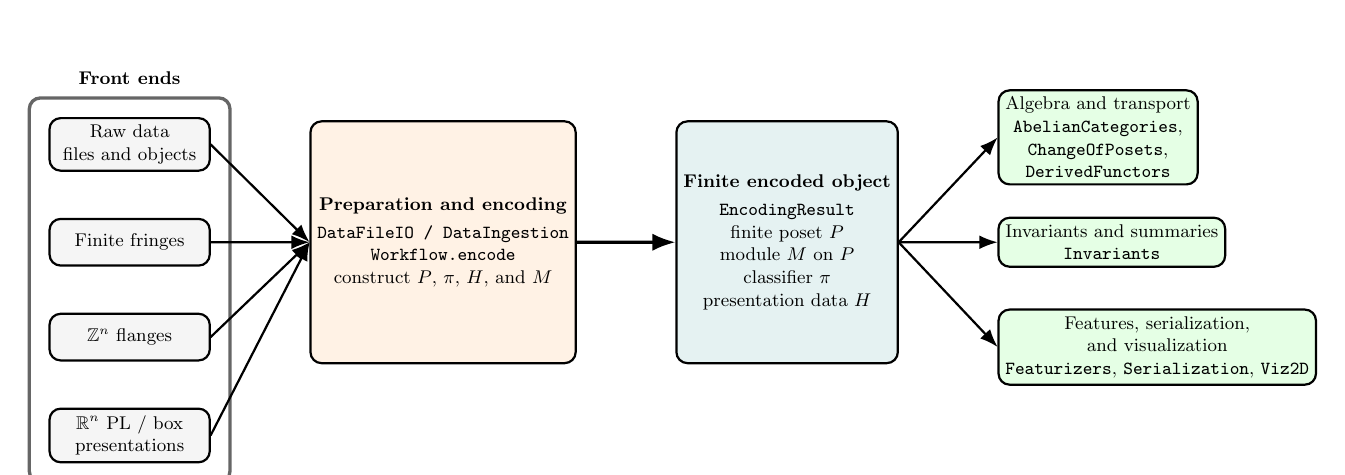
\begin{tikzpicture}[
    >=Latex,
    scale=0.74,
    transform shape,
    node distance=8mm and 10mm,
    every node/.style={font=\small},
    src/.style={rounded corners, draw, thick, align=center, minimum width=2.75cm, minimum height=0.8cm, fill=gray!8},
    stage/.style={rounded corners, draw, thick, align=center, minimum width=3.8cm, minimum height=1.0cm, fill=orange!10},
    outbox/.style={rounded corners, draw, thick, align=center, minimum width=3.0cm, minimum height=0.82cm, fill=green!10},
    layer/.style={rounded corners, draw=black!60, very thick, inner sep=7pt}
]

\node[src] (raw) {Raw data\\files and objects};
\node[src, below=of raw] (finite) {Finite fringes};
\node[src, below=of finite] (flange) {$\mathbb{Z}^n$ flanges};
\node[src, below=of flange] (pl) {$\mathbb{R}^n$ PL / box\\presentations};
\node[layer, fit=(raw)(finite)(flange)(pl), label={[yshift=0.2em]above:\textbf{Front ends}}] {};

\node[stage, right=17mm of finite, minimum height=4.15cm] (encode) {
\textbf{Preparation and encoding}\\[0.3em]
\texttt{DataFileIO / DataIngestion}\\
\texttt{Workflow.encode}\\
construct $P$, $\pi$, $H$, and $M$
};

\node[stage, right=17mm of encode, minimum height=4.15cm, fill=teal!10] (result) {
\textbf{Finite encoded object}\\[0.3em]
\texttt{EncodingResult}\\
finite poset $P$\\
module $M$ on $P$\\
classifier $\pi$\\
presentation data $H$
};

\node[outbox, right=17mm of result, yshift=18mm] (alg) {Algebra and transport\\\texttt{AbelianCategories},\\\texttt{ChangeOfPosets},\\\texttt{DerivedFunctors}};
\node[outbox, right=17mm of result] (inv) {Invariants and summaries\\\texttt{Invariants}};
\node[outbox, right=17mm of result, yshift=-18mm] (feat) {Features, serialization,\\and visualization\\\texttt{Featurizers}, \texttt{Serialization}, \texttt{Viz2D}};

\draw[->, thick] (raw.east) -- (encode.west);
\draw[->, thick] (finite.east) -- (encode.west);
\draw[->, thick] (flange.east) -- (encode.west);
\draw[->, thick] (pl.east) -- (encode.west);
\draw[->, very thick] (encode.east) -- (result.west);
\draw[->, thick] (result.east) -- (alg.west);
\draw[->, thick] (result.east) -- (inv.west);
\draw[->, thick] (result.east) -- (feat.west);

\end{tikzpicture}
\caption{An architectural overview of \TAMER. Multiple front end representations are funneled through a finite encoding step, after which a common finite-poset module supports algebraic, invariant, workflow, and visualization tasks.}
\label{fig:system-overview}
\end{figure}

Figure~\ref{fig:intro-architecture} summarizes this thesis-level perspective. The picture is deliberately asymmetric. The left side contains many input formats because the system is meant to meet users where their data or mathematical models already live. The middle stage is narrow because encoding is a single conceptual move: build a finite region poset and a classifier that factor the ambient module through it. The right side then branches outward again because, once the finite-poset representation exists, a wide range of algebraic and applied computations become available from the same object.

The asymmetry of this diagram is deliberate.  The left side is diverse because the library is intended to accept front-end objects in the form most natural to their source.  The middle is narrow because there is only one conceptual move that matters: build a finite encoding.  The right side branches again because, once the encoded object exists, many different computational goals can be pursued from the same internal representation.

\subsection{Architectural layering}

The implementation follows this conceptual organization closely.  At the bottom lies a runtime and linear-algebra layer.  The role of this layer is not only to provide matrix kernels, but to provide \emph{exact} and backend-aware matrix kernels, together with caches and autotuned thresholds, so that later algebraic code can be written at the level of modules rather than at the level of ad hoc numerical special cases.  In the present codebase this role is played chiefly by the \texttt{CoreModules} and \texttt{FieldLinAlg} families.

Above that lies the finite-poset representation layer.  This is the layer in which finite posets, upsets, downsets, fringe modules, finite-poset modules, abelian-category constructions, and indicator resolutions are represented concretely.  Conceptually, this is the algebraic core of the system.  Once an object has reached this layer, ordinary linear algebra and functor-category algebra can be applied directly.  The modules \texttt{FiniteFringe}, \texttt{Modules}, \texttt{AbelianCategories}, and \texttt{IndicatorResolutions} occupy this level.

The encoding layer sits above the representation layer and below the user-facing workflow.  Its job is to build finite region posets and classifier maps from front-end objects over $\mathbb{Z}^n$ or $\mathbb{R}^n$, together with any compiled or cached structures needed for efficient point location and pushforward.  This is where the library's main differentiating algorithms live.  In the current codebase, the relevant families are \texttt{EncodingCore}, \texttt{ZnEncoding}, \texttt{PLBackend}, and \texttt{PLPolyhedra}.

Then comes the orchestration layer.  Rather than exposing every internal constructor directly to ordinary users, \TAMER{} organizes common workflows through a small number of stable entry points.  The key example is \texttt{Workflow.encode}, which converts a front-end object into an \texttt{EncodingResult}.  Similar wrappers then dispatch to homological algebra, invariants, and comparison routines.  The \texttt{Results} layer is important here because it carries not only the encoded mathematical object but also options, provenance, backend choice, and metadata.

Finally, several cross-cutting layers operate in parallel with the main algebraic pipeline.  The ingestion layer bridges raw data and formal presentations.  The serialization layer makes front ends, encodings, and feature artifacts reproducible.  The featurization layer treats encoded modules as reusable objects in statistical and machine-learning workflows.  The visualization layer treats the same encoded objects as the basis for exploration and explanation.  These are not auxiliary conveniences added after the mathematical design was fixed.  They are part of what it means for the encoded module to serve as a stable internal language across the whole system.

\subsection{Why the finite encoding step is the organizing principle}

The central architectural claim of this thesis can be stated in a mathematically precise form.

\begin{proposition}[Encoding as a computational boundary]
Let $\mathcal{I}$ be any class of pre-encoding objects for which the library constructs an encoding result
\[
E(X)=(P_X,M_X,\pi_X,H_X)
\]
with $P_X$ finite and $M_X$ a finite-poset module on $P_X$.  Let $F$ be any construction defined functorially on finite-poset modules, or on finite-poset modules together with their associated encoding maps when ambient evaluation is required.  Then the workflow value associated to $X$ and $F$ depends on $X$ only through $E(X)$.
\end{proposition}

\begin{proof}
By design, every downstream routine in the system receives the encoded module $M_X$, and when necessary the classifier $\pi_X$ or presentation data $H_X$, rather than the original front-end object.  Once the encoding result has been constructed, subsequent computation is performed entirely against that finite package.  Therefore the value of any later functorial construction depends only on the encoding result.
\end{proof}

This proposition is almost tautological, but that is exactly the point.  It identifies the precise place at which the computational problem changes character.  Before encoding, one is still dealing with ambient parameter spaces, geometric representations, filtration choices, and presentation-specific subtleties.  After encoding, one is dealing with a finite-poset module.  The post-encoding world is therefore uniform even though the pre-encoding world is intentionally heterogeneous.

Two consequences are especially important.  First, the library can support many front ends without fragmenting into unrelated subsystems.  Finite fringes, flanges, PL presentations, and ingested data all converge to the same encoded module language.  Second, expensive infrastructure can be concentrated where it matters most.  Exact linear algebra, caches, resolution builders, and change-of-poset routines only need to be implemented once for the finite-poset world, because every other front end is designed to arrive there.

This is also the main mathematical reason that \TAMER{} can do things that are awkward or impossible for libraries built around summary-first architectures.  Once a genuine encoded module has been retained, one may compute kernels, cokernels, equalizers, pushouts, projective and injective approximations, derived functors, and comparison transports before one ever decides which invariant or feature vector to extract.  The module is therefore not a transient intermediate artifact.  It is the central object around which the rest of the pipeline is organized.

\subsection{Road map for the remainder of the thesis}

The rest of the thesis follows the same order as the pipeline itself.  The next chapter studies pre-encoding objects and data interfaces.  After that, the thesis turns to the encoding step proper, which is the mathematical and algorithmic center of the work.  Once the encoding machinery has been established, the following chapters discuss what becomes possible after encoding: homological algebra on finite posets, derived functors, invariants, summary layers, serialization, featurization, visualization, and finally benchmark evidence for the tractability and competitiveness of the whole workflow.

Subsequent chapters then move in the same direction as Figure~\ref{fig:intro-architecture}: from pre-encoding representations and data ingestion, to the encoding algorithms themselves, to the algebra, invariants, workflow layers, visualization support, and finally benchmarks. The order is deliberate. The thesis argues that nearly every distinctive feature of the library is best understood not as an isolated implementation trick, but as a consequence of making the finite encoding step explicit and central.

This organization is intentional.  It mirrors the main claim of the thesis.  The library is best understood not as a loose collection of algorithms, but as a system whose varied capabilities are all consequences of one choice: make finite encoding explicit, robust, and central.


\section{Bibliography}\label{app:bibliography-notes}


\begin{thebibliography}{99}

\bibitem[Mil20]{Mil20}
E.~Miller.
\newblock \emph{Homological algebra of modules over posets}.
\newblock \href{https://arxiv.org/abs/2008.00063}{arXiv:2008.00063}, 2020.

\bibitem[Waa24]{Waa24}
L.~Waas.
\newblock \emph{Notes on abelianity of categories of finitely encodable persistence modules}.
\newblock \href{https://arxiv.org/abs/2407.08666}{arXiv:2407.08666}, 2024.

\bibitem[Mil23]{Mil23}
E.~Miller.
\newblock \emph{Stratifications of real vector spaces from constructible sheaves with conical microsupport}.
\newblock \emph{Journal of Applied and Computational Topology}, 7(3):473--489, 2023.
\newblock \href{https://doi.org/10.1007/s41468-023-00112-1}{doi:10.1007/s41468-023-00112-1}.

\bibitem[KS18]{KS18}
M.~Kashiwara and P.~Schapira.
\newblock \emph{Persistent homology and microlocal sheaf theory}.
\newblock \emph{Journal of Applied and Computational Topology}, 2(1--2):83--113, 2018.
\newblock \href{https://arxiv.org/abs/1705.00955}{arXiv:1705.00955}.

\bibitem[CB15]{CB15}
W.~Crawley-Boevey.
\newblock \emph{Decomposition of pointwise finite-dimensional persistence modules}.
\newblock \emph{Journal of Algebra and Its Applications}, 14(5):1550066, 2015.
\newblock \href{https://doi.org/10.1142/S0219498815500668}{doi:10.1142/S0219498815500668}.

\bibitem[ZC05]{ZC05}
A.~Zomorodian and G.~Carlsson.
\newblock \emph{Computing persistent homology}.
\newblock \emph{Discrete \& Computational Geometry}, 33:249--274, 2005.
\newblock \href{https://doi.org/10.1007/s00454-004-1146-y}{doi:10.1007/s00454-004-1146-y}.

\bibitem[CZ09]{CZ09}
G.~Carlsson and A.~Zomorodian.
\newblock \emph{The theory of multidimensional persistence}.
\newblock \emph{Discrete \& Computational Geometry}, 42:71--93, 2009.
\newblock \href{https://doi.org/10.1007/s00454-009-9176-0}{doi:10.1007/s00454-009-9176-0}.

\bibitem[CEH07]{CEH07}
D.~Cohen-Steiner, H.~Edelsbrunner, and J.~Harer.
\newblock \emph{Stability of persistence diagrams}.
\newblock \emph{Discrete \& Computational Geometry}, 37(1):103--120, 2007.
\newblock \href{https://doi.org/10.1007/s00454-006-1276-5}{doi:10.1007/s00454-006-1276-5}.

\bibitem[ELZ02]{ELZ02}
H.~Edelsbrunner, D.~Letscher, and A.~Zomorodian.
\newblock \emph{Topological persistence and simplification}.
\newblock \emph{Discrete \& Computational Geometry}, 28:511--533, 2002.
\newblock \href{https://doi.org/10.1007/s00454-002-2885-2}{doi:10.1007/s00454-002-2885-2}.

\bibitem[Les15]{Les15}
M.~Lesnick.
\newblock \emph{The theory of the interleaving distance on multidimensional persistence modules}.
\newblock \emph{Foundations of Computational Mathematics}, 15(3):613--650, 2015.
\newblock \href{https://doi.org/10.1007/s10208-015-9255-y}{doi:10.1007/s10208-015-9255-y}.

\bibitem[LW15]{LW15}
M.~Lesnick and M.~Wright.
\newblock \emph{Interactive visualization of 2-D persistence modules}.
\newblock \href{https://arxiv.org/abs/1512.00180}{arXiv:1512.00180}, 2015.

\bibitem[RIVET]{RIVET}
M.~Lesnick and M.~Wright.
\newblock \emph{RIVET: The rank invariant visualization and exploration tool} (software).
\newblock \url{https://github.com/rivetTDA/rivet}.

\bibitem[LS24]{LS24}
D.~Loiseaux and H.~Schreiber.
\newblock \emph{multipers: Multiparameter persistence for machine learning}.
\newblock \emph{Journal of Open Source Software}, 9(103):6773, 2024.
\newblock \href{https://doi.org/10.21105/joss.06773}{doi:10.21105/joss.06773}.

\bibitem[CDSGO16]{CDSGO16}
F.~Chazal, V.~de~Silva, M.~Glisse, and S.~Y. Oudot.
\newblock \emph{The Structure and Stability of Persistence Modules}.
\newblock SpringerBriefs in Mathematics. Springer, 2016.
\newblock \href{https://doi.org/10.1007/978-3-319-42545-0}{doi:10.1007/978-3-319-42545-0}.

\bibitem[Oud15]{Oud15}
S.~Y. Oudot.
\newblock \emph{Persistence Theory: From Quiver Representations to Data Analysis}.
\newblock Mathematical Surveys and Monographs, Vol.~209. American Mathematical Society, 2015.

\bibitem[EH10]{EH10}
H.~Edelsbrunner and J.~L. Harer.
\newblock \emph{Computational Topology: An Introduction}.
\newblock American Mathematical Society, 2010.

\bibitem[Mac98]{Mac98}
S.~Mac~Lane.
\newblock \emph{Categories for the Working Mathematician}.
\newblock Graduate Texts in Mathematics, Vol.~5. Springer, 2nd edition, 1998.
\newblock \href{https://doi.org/10.1007/978-1-4757-4721-8}{doi:10.1007/978-1-4757-4721-8}.

\bibitem[Wei94]{Wei94}
C.~A. Weibel.
\newblock \emph{An Introduction to Homological Algebra}.
\newblock Cambridge Studies in Advanced Mathematics, Vol.~38. Cambridge University Press, 1994.

\bibitem[Eis95]{Eis95}
D.~Eisenbud.
\newblock \emph{Commutative Algebra with a View Toward Algebraic Geometry}.
\newblock Graduate Texts in Mathematics, Vol.~150. Springer, 1995.
\newblock \href{https://doi.org/10.1007/978-1-4612-5350-1}{doi:10.1007/978-1-4612-5350-1}.

\bibitem[MS05]{MS05}
E.~Miller and B.~Sturmfels.
\newblock \emph{Combinatorial Commutative Algebra}.
\newblock Graduate Texts in Mathematics, Vol.~227. Springer, 2005.
\newblock \href{https://doi.org/10.1007/b138602}{doi:10.1007/b138602}.

\end{thebibliography}

\end{document}
